\chapter{Study and realization of the Sprint 3}
\minitoc
\newpage

\setcounter{secnumdepth}{2} % Resume counting the sections for the toc with a depth of 2 (Sections and sub-sections)
% ----------------------------------- SECTIONS (v) ----------------------------------- %
% ----------------------- Deployment process ----------------------- %
\section{Backlog of the sprint}
In this sprint, the focus shifts towards enhancing the job description definition feature and facilitating better communication of the defined job descriptions.

In Sprint 3, we are building upon the job description definition feature developed in Sprint 2, adding additional capabilities that make it more useful and convenient for the HR Managers. They can now easily share the job descriptions they've defined, either by emailing them directly to candidates or by printing them to PDF for offline use. This completes the main functionality of the job description definition feature and enhances its utility for the end users.

\begin{xltabular}{1.2\textwidth}{
        | >{\hsize=0.8\hsize\raggedright\arraybackslash}X
        | >{\hsize=0.8\hsize\raggedright\arraybackslash}X
        | >{\hsize=1.8\hsize\raggedright\arraybackslash}X
        | >{\hsize=0.6\hsize\raggedright\arraybackslash}X |}
    \caption{Sprint 2 Backlog} \\
    \hline
    \rowcolor{primary} \textbf{User Story} & \textbf{Subtask} & \textbf{Description} & \textbf{Estimated Time} \\
    \hline
    \endfirsthead
    \multicolumn{4}{c}%
    {\tablename\ \thetable\ -- \textit{Continued from previous page}} \\
    \hline
    \rowcolor{primary} \textbf{User Story} & \textbf{Subtask} & \textbf{Description} & \textbf{Estimated Time} \\
    \hline
    \endhead
    \hline \multicolumn{4}{r}{\textit{Continued on next page}} \\
    \endfoot
    \hline
    \endlastfoot
    % Your table content here
    User Story 1: As an HR Manager, I want to email the generated job description to potential candidates directly from the system. & Subtask 1.1: Develop a process to email job descriptions & This involves creating a mechanism that allows the system to send emails with the generated job description. & 5 days \\
    \hline
    & Subtask 1.2: Implement the process in the system & This involves integrating the emailing mechanism into the existing system and ensuring it functions correctly with the job description generation feature.  & 2 days \\
    \hline
    User Story 2: As an HR Manager, I want to print the nested skills and tasks to a PDF format for documentation or offline use. & Subtask 2.1: Develop a process to convert selected skills and tasks to a PDF & This involves creating a mechanism that allows the system to export the selected skills and tasks into a PDF file. & 3 days \\
    \hline
    & Subtask 2.2: Implement the process in the system & This involves integrating the PDF export mechanism into the existing system and ensuring it functions correctly with the job description generation feature. & 2 days \\
    \hline
    User Story 3: As an HR Manager, I want to interact with a chatbot to understand the system better and get guidance on the process. & Subtask 3.1: Develop a chatbot using GPT-3 & This involves designing and developing a chatbot that can interact with the users and provide guidance on using the system. & 1 week \\
    \hline
    & Subtask 3.2: Integrate the chatbot into the system & This involves integrating the chatbot into the existing system and ensuring it interacts correctly with the users. & 2 days \\
    \hline
\end{xltabular}


\newpage
\section{Functional Specification}
In this sub-section, we present the analysis phase that answers the question “what does the system do”. The answer to this question is translated by the presentation of the diagram of the use cases and the textual description of each of them.

\subsection{Use Case Diagram}
The use case would typically include the following main actors and their interactions with the system :

\begin{figure}[H]
    \centering
    \makebox[\textwidth]{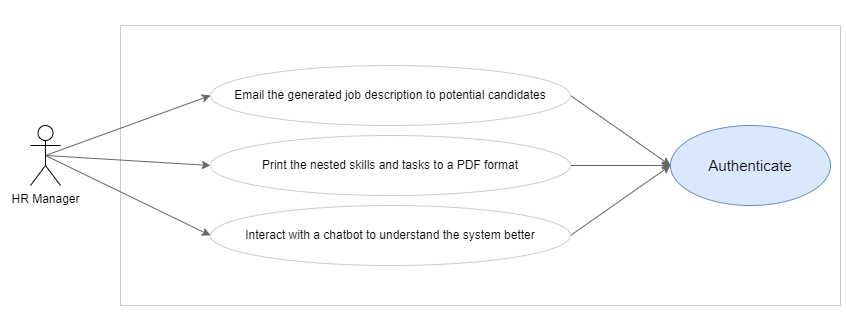
\includegraphics[width=\linewidth]{src/assets/images/HRMUseCase3.drawio.png}}
    \caption{ Use Case Diagram For Sprint 3 }
    \label{fig:Sprint3_UseCaseDiagram}
\end{figure}

\subsection{Textual Description of the Use Cases}
\subsubsection{\underline{Use Case 1 : Email the Generated Job Description}}
In this use case, the HR Manager uses the system to email the generated job description directly to potential candidates. This action enhances the utility of the job description creation process as it provides a direct communication link with potential candidates. After successfully generating a job description, the HR Manager selects the option to email the job description. The system asks the HR Manager to provide the email addresses of the potential candidates. Upon confirmation, the system sends the job description to the given email addresses. This allows the HR Manager to communicate the job description without leaving the system, streamlining the job advertising process.

\renewcommand{\arraystretch}{1.5}
\setlength{\tabcolsep}{10pt}

\begin{table}[H]
    \renewcommand{\arraystretch}{1.5}%
    \caption{Use Case 1 : Email the Generated Job Description}
    \centering
    \medskip
    \small
    \begin{tabularx}{1.2\textwidth} {
            | >{\hsize=0.4\hsize\raggedright\arraybackslash}X
            | >{\hsize=1.6\hsize\raggedright\arraybackslash}X |}
        \hline
        \textbf{Title}                 & Email the Generated Job Description                                                                                               \\
        \hline
        \textbf{Main Actor}            & HR Manager                                                                                                                        \\
        \hline
        \textbf{Summary}               & The HR Manager uses the system to email the generated job description directly to potential candidates.                           \\
        \hline
        \textbf{Preconditions}         & - A job description has been generated by the system.                                                                             \\
                                       & - The HR Manager has the email addresses of the potential candidates.                                                             \\
        \hline
        \textbf{Main Success Scenario} & 1. HR Manager selects the option to email the job description.                                                                    \\
                                       & 2. HR Manager enters the email addresses of the potential candidates.                                                             \\
                                       & 3. HR Manager confirms the action.                                                                                                \\
                                       & 4. The system sends the job description to the provided email addresses.                                                          \\
        \hline
        \textbf{Postconditions}        & - The generated job description has been emailed to the potential candidates.                                                     \\
        \hline
        \textbf{Alternative Scenarios} & - If the HR Manager enters an invalid email address, the system should notify the HR Manager and ask for a correct email address. \\
        \hline
    \end{tabularx}
    \normalsize
\end{table}



\subsubsection{\underline{Use case 2: Print the Nested Skills and Tasks to a PDF}}
This use case concerns the conversion of selected skills and tasks into a PDF document. This feature facilitates the documentation and offline use of the information gathered during the job description creation process. The HR Manager, after choosing the necessary skills and tasks, selects the option to print this data to a PDF. The system processes this request and produces a PDF document containing the selected skills and tasks. The HR Manager can then decide to save this PDF for future reference or print it for offline usage. This feature is especially useful for keeping track of decision-making processes and providing offline or hard copy resources during recruitment exercises.

\begin{table}[H]
    \renewcommand{\arraystretch}{1.5}%
    \caption{Use Case 2 : Print the Nested Skills and Tasks to a PDF}
    \centering
    \medskip
    \small
    \begin{tabularx}{1.2\textwidth} {
            | >{\hsize=0.4\hsize\raggedright\arraybackslash}X
            | >{\hsize=1.6\hsize\raggedright\arraybackslash}X |}
        \hline
        \textbf{Title}                 & Print the Nested Skills and Tasks to a PDF                                                                                  \\
        \hline
        \textbf{Main Actor}            & HR Manager                                                                                                                  \\
        \hline
        \textbf{Summary}               & The HR Manager uses the system to convert the selected skills and tasks into a PDF format for documentation or offline use. \\
        \hline
        \textbf{Preconditions}         & - The HR Manager has selected specific skills and tasks for a job description.                                              \\
                                       & - The system has the capability to generate PDF files.                                                                      \\
        \hline
        \textbf{Main Success Scenario} & 1. HR Manager selects the option to print the skills and tasks to a PDF.                                                    \\
                                       & 2. The system converts the selected skills and tasks into a PDF format.                                                     \\
                                       & 3. The HR Manager saves or prints the PDF for documentation or offline use.                                                 \\
        \hline
        \textbf{Postconditions}        & The selected skills and tasks have been printed to a PDF.                                                                   \\
        \hline
        \textbf{Alternative Scenarios} & - If the system fails to generate the PDF, the HR Manager should be notified about the error.                               \\
        \hline
    \end{tabularx}
    \normalsize
\end{table}

\subsubsection{\underline{Use Case 3: Interact with a Chatbot for Guidance}}
This use case describes the interaction of the HR Manager with a chatbot designed and developed using GPT-3. The purpose of this feature is to provide the HR Manager with on-the-spot guidance about the system and the job description creation process. The HR Manager opens the chatbot and proceeds to ask questions. The chatbot, backed by the capabilities of GPT-3, provides responses that aim to address the HR Manager's questions accurately. This interaction continues until the HR Manager is satisfied with the information provided. This feature enriches the user experience by providing immediate assistance and guidance, increasing the system's usability and effectiveness.


\begin{table}[H]
    \renewcommand{\arraystretch}{1.5}%
    \caption{Use Case 3 : Interact with a Chatbot for Guidance}
    \centering
    \medskip
    \small
    \begin{tabularx}{1.2\textwidth} {
            | >{\hsize=0.4\hsize\raggedright\arraybackslash}X
            | >{\hsize=1.6\hsize\raggedright\arraybackslash}X |}
        \hline
        \textbf{Title}                 & Interact with a Chatbot for Guidance                                                                                   \\
        \hline
        \textbf{Main Actor}            & HR Manager                                                                                                             \\
        \hline
        \textbf{Summary}               & The HR Manager interacts with a chatbot in the system to better understand the system and get guidance on the process. \\
        \hline
        \textbf{Preconditions}         & - The system has a chatbot feature.                                                                                    \\
                                       & - The chatbot has been designed and developed using GPT-3.                                                             \\
        \hline
        \textbf{Main Success Scenario} & 1. HR Manager opens the chatbot in the system.                                                                         \\
                                       & 2. HR Manager asks the chatbot questions about the system or the job description process.                              \\
                                       & 3. The chatbot provides responses and guidance to the HR Manager based on its design and development.                  \\
                                       & 4. The HR Manager continues to interact with the chatbot until they have the information they need.                    \\
        \hline
        \textbf{Postconditions}        & The HR Manager has interacted with the chatbot and received guidance on the system and the process.                    \\
        \hline
        \textbf{Alternative Scenarios} & - If the chatbot does not understand the HR Manager's question, it should ask for clarification or rephrasing.         \\
                                       & - If the chatbot provides incorrect or unclear guidance, the HR Manager should have the option to report the issue.    \\
        \hline
    \end{tabularx}
    \normalsize
\end{table}

\section{Design}
In this sub-section, we will present the different detailed Activity Diagrams + Sequence diagrams for the first sprint.

\newpage
\subsection{Detailed Activity Diagrams}
\subsubsection{Use Case 1 : Email the Generated Job Description}


\begin{figure}[H]
    \centering
    \makebox[\textwidth]{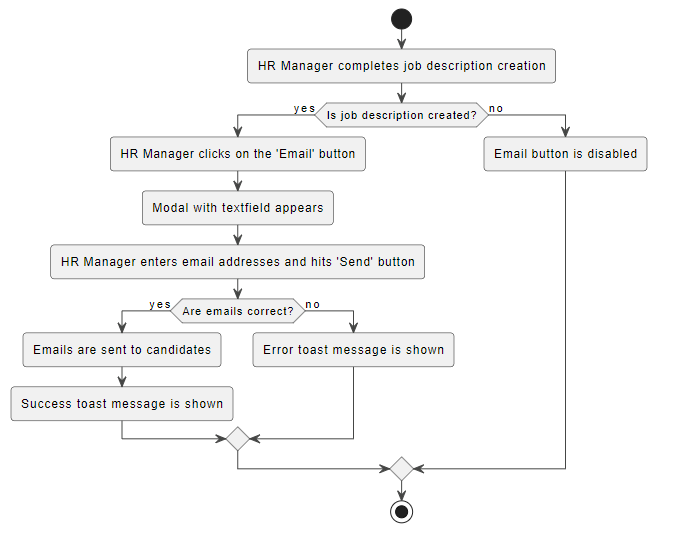
\includegraphics[width=1\linewidth]{src/assets/images/sprint3UseCase1.png}}
    \caption{ Activity Diagram for the Email the Generated Job Description Use-Case }
    \label{fig:UseCase1Sprint3_Activity_Diagram}
\end{figure}

\subsection*{Description}
\begin{enumerate}
    \item We start from the point where the HR Manager completes the job description creation process, described in detail in a previous use case.
    \item If the job description is successfully created, the HR Manager can click on the "Email" button. This triggers a modal with a textfield to appear.
    \item The HR Manager enters the email addresses of the candidates into this textfield and hits "Send".
    \item If the email addresses are valid, the emails are sent to the candidates, and a success toast message is shown.
    \item If the email addresses are not valid, an error toast message is shown.
    \item If the job description creation is not completed or successful, the "Email" button remains disabled.
\end{enumerate}


\subsubsection{Use Case 2 : Print the Nested Skills and Tasks to a PDF}


\begin{figure}[H]
    \centering
    \makebox[\textwidth]{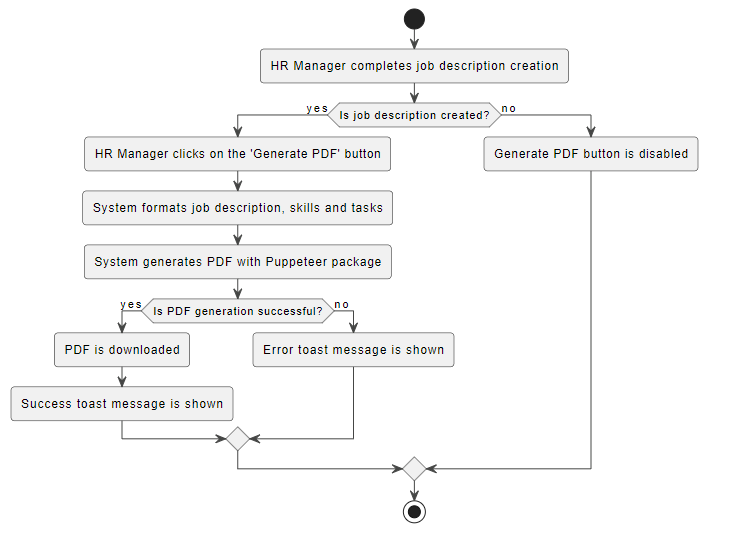
\includegraphics[width=1\linewidth]{src/assets/images/sprint3UseCase2.png}}
    \caption{ Activity Diagram for the Print the Nested Skills and Tasks to a PDF Use-Case }
    \label{fig:UseCase2Sprint3_Activity_Diagram}
\end{figure}

\subsection*{Description}
\begin{enumerate}
    \item After job description completion, the HR Manager initiates the process, allowing "Generate PDF" activation upon success.
    \item This button triggers system to format necessary details and Puppeteer generates a PDF.
    \item Success or failure leads to respective messages; failure or incomplete descriptions disable PDF generation.
\end{enumerate}



\subsubsection{Use Case 3: Interact with a Chatbot for Guidance}


\begin{figure}[H]
    \centering
    \makebox[\textwidth]{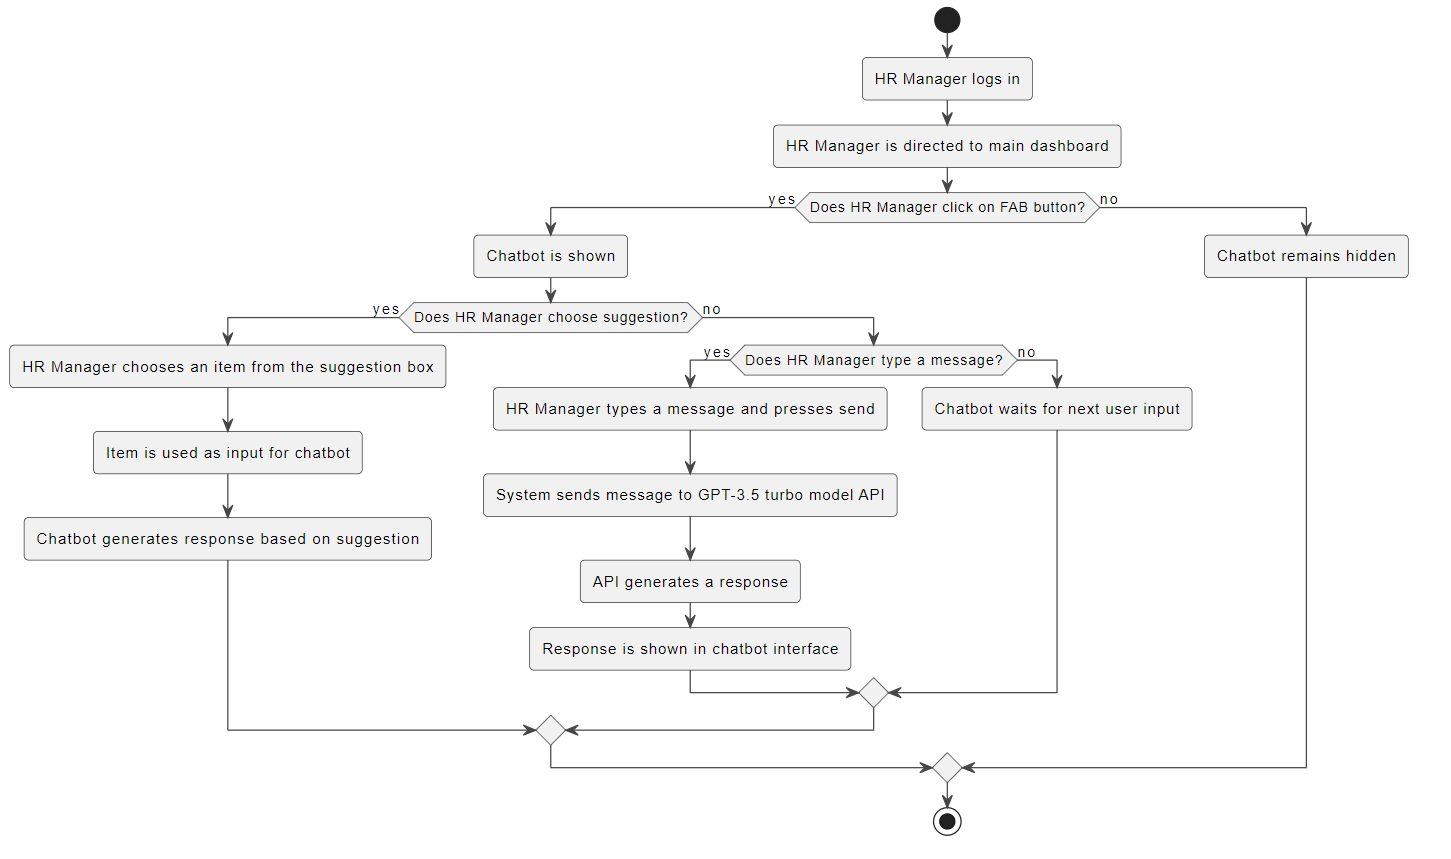
\includegraphics[width=1.25\linewidth]{src/assets/images/sprint3UseCase3.png}}
    \caption{ Activity Diagram for the Interact with a Chatbot for Guidance Use-Case }
    \label{fig:UseCase3Sprint3_Activity_Diagram}
\end{figure}

\subsection*{Description}
\begin{enumerate}
    \item Activity begins with HR Manager login and redirection to main dashboard.
    \item Clicking the FAB button reveals the chatbot interface.
    \item Choosing a suggestion prompts a chatbot response based on the selected item.
    \item Alternatively, typing and sending a message results in a response from the GPT-3.5 Turbo API.
    \item Absence of a message or selection leaves the chatbot awaiting input.
    \item If the FAB button is unclicked, the chatbot stays hidden.
\end{enumerate}

\newpage
\subsection{Detailed Sequence Diagrams}
\subsubsection{Use Case 1 : Email the Generated Job Description} 

\begin{figure}[H]
    \centering
    \makebox[\textwidth]{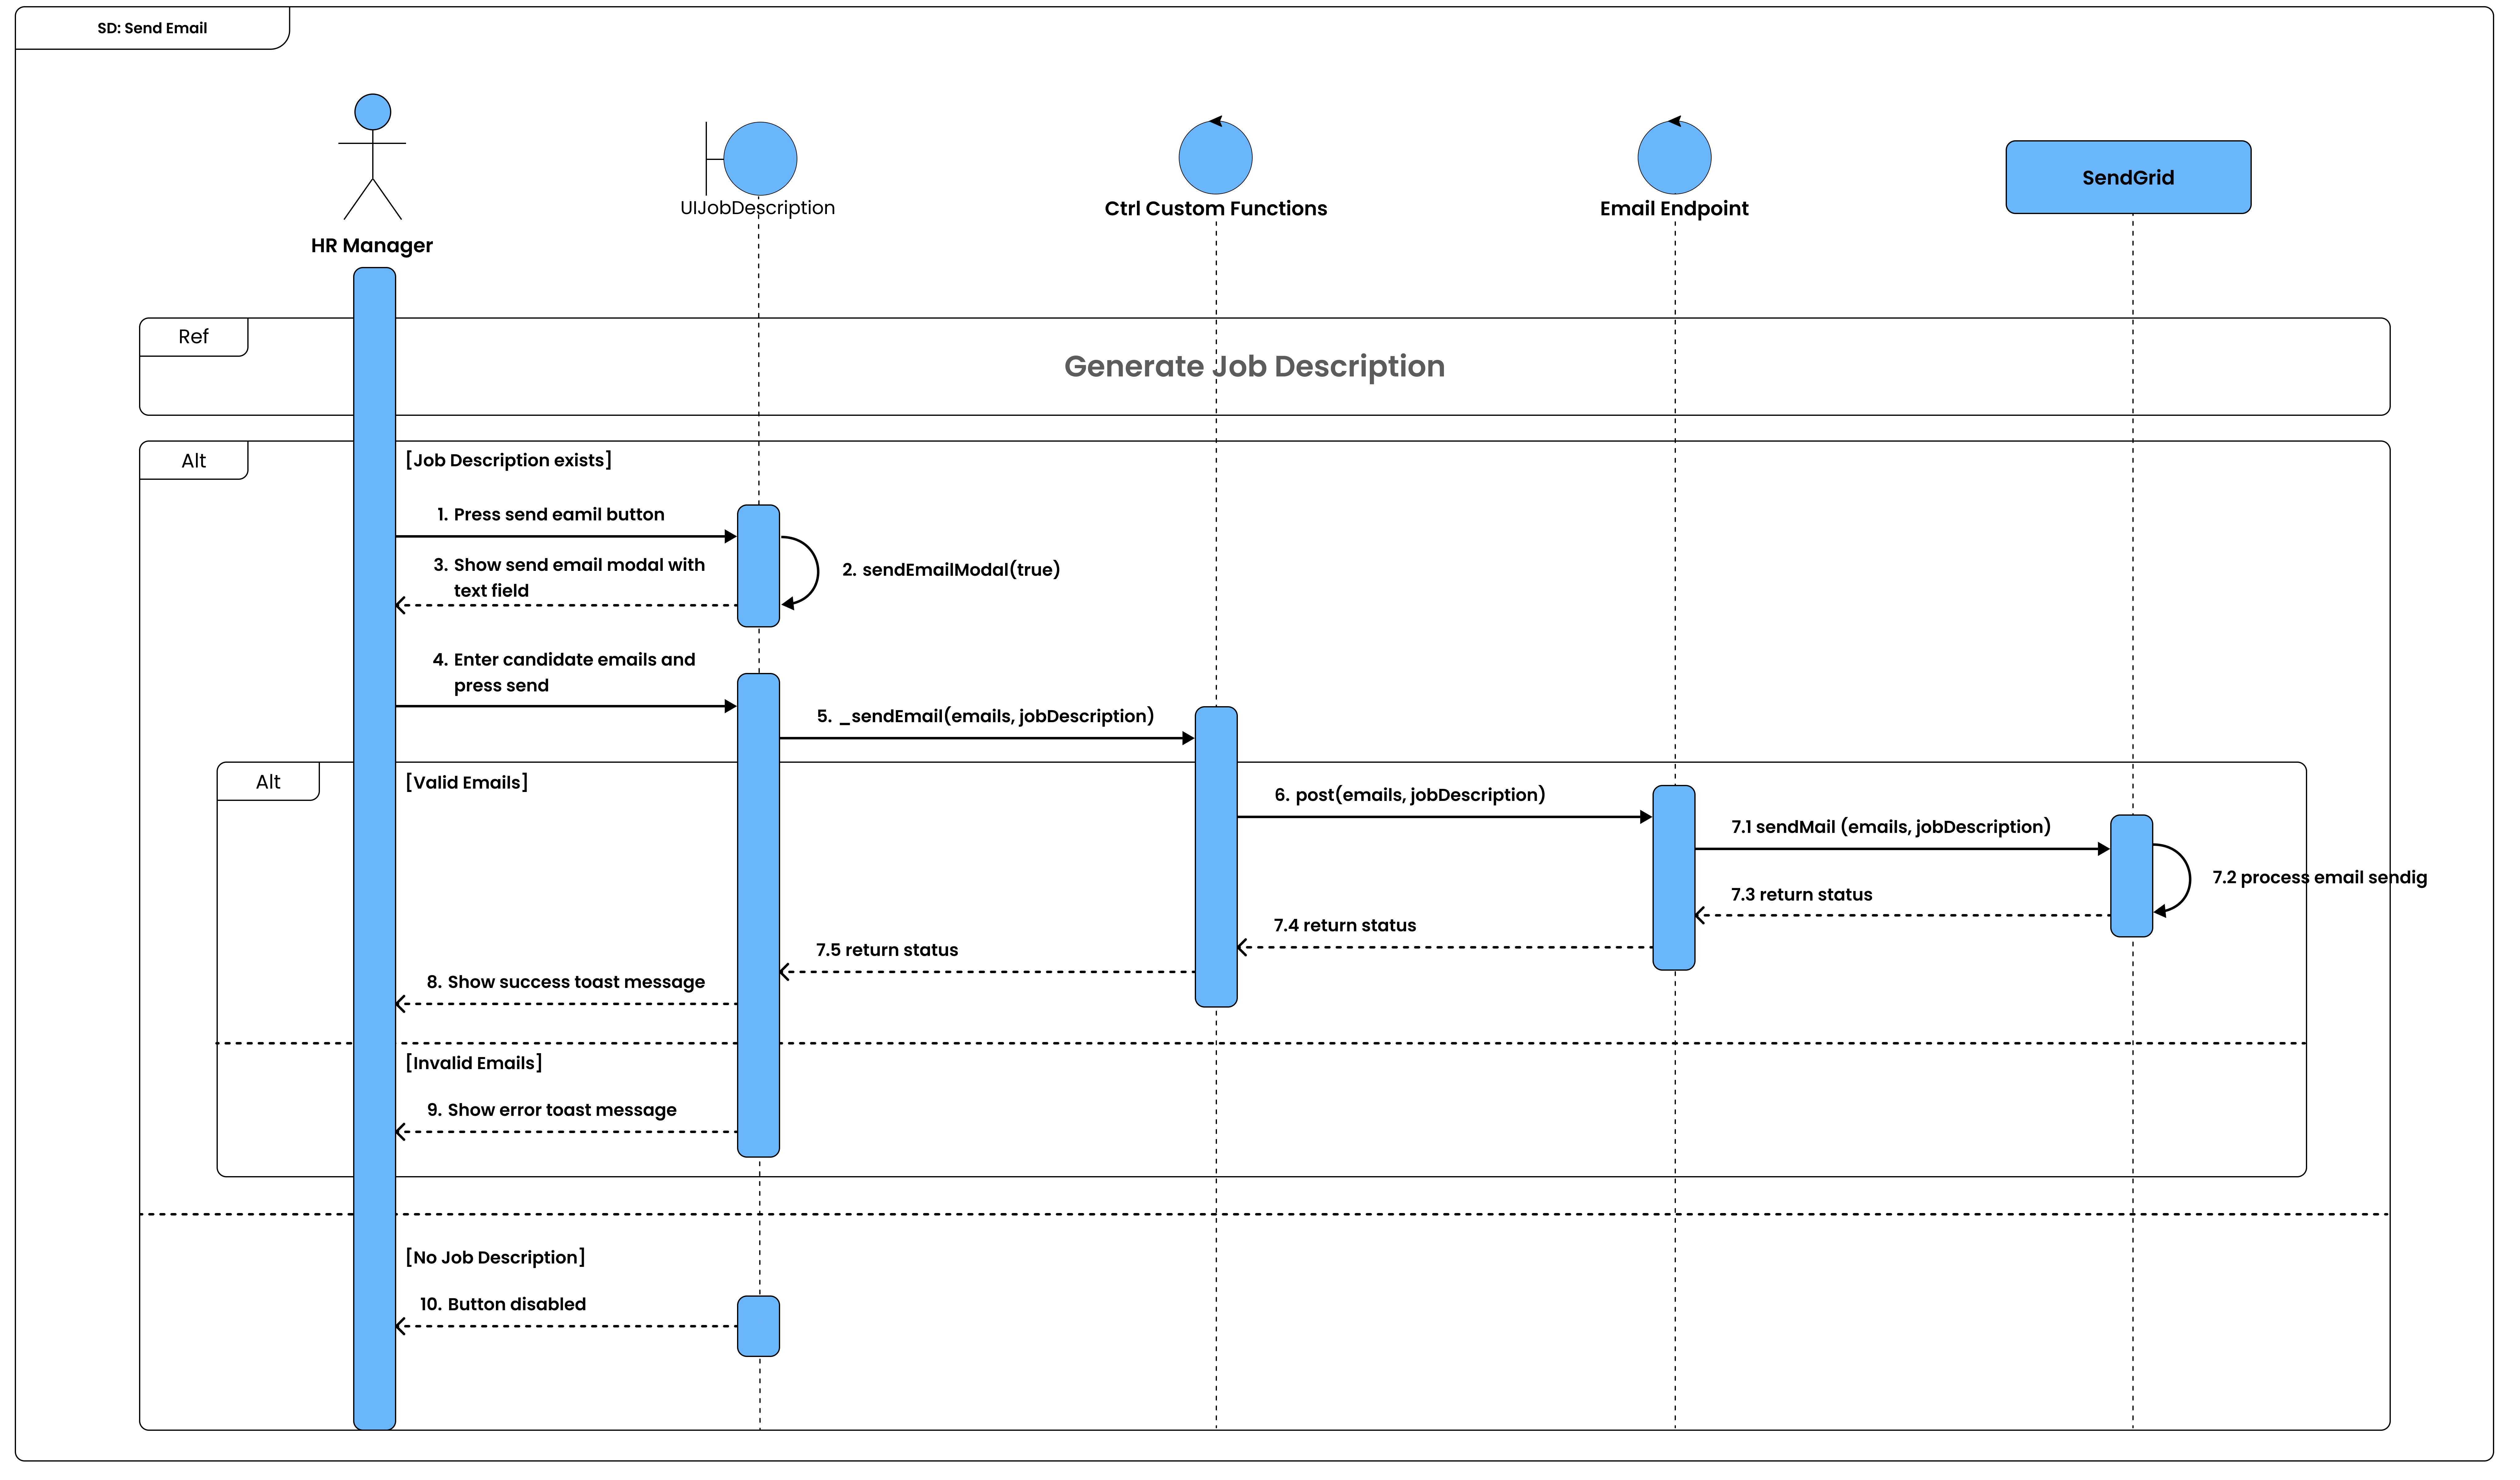
\includegraphics[width=1.25\linewidth]{src/assets/images/SD-Send-Email.jpg}}
    \caption{ Sequence Diagram for the Email the Generated Job Description Use-Case }
    \label{fig:UseCase1Sprint3_Sequence_Diagram}
\end{figure}

\subsection*{Description}
In this sequence diagram, the HR Manager initiates the process by clicking the "Send Email" button on the UI. This triggers the display of a modal for entering email addresses. Once the desired email addresses are provided, the manager hits 'Send'. A function is then triggered to validate the entered emails.

If the emails are valid, an HTTP request is made to a web service hosted on Render. The service takes the job description and emails, then interacts with SendGrid platform via an API call. SendGrid sends the emails using the provided details and template. Upon successful transmission, a toast notification is displayed on the FlutterFlow UI, confirming the successful dispatch of the emails.


\subsubsection{Use Case 2: Print the Nested Skills and Tasks to a PDF} 

\begin{figure}[H]
    \centering
    \makebox[\textwidth]{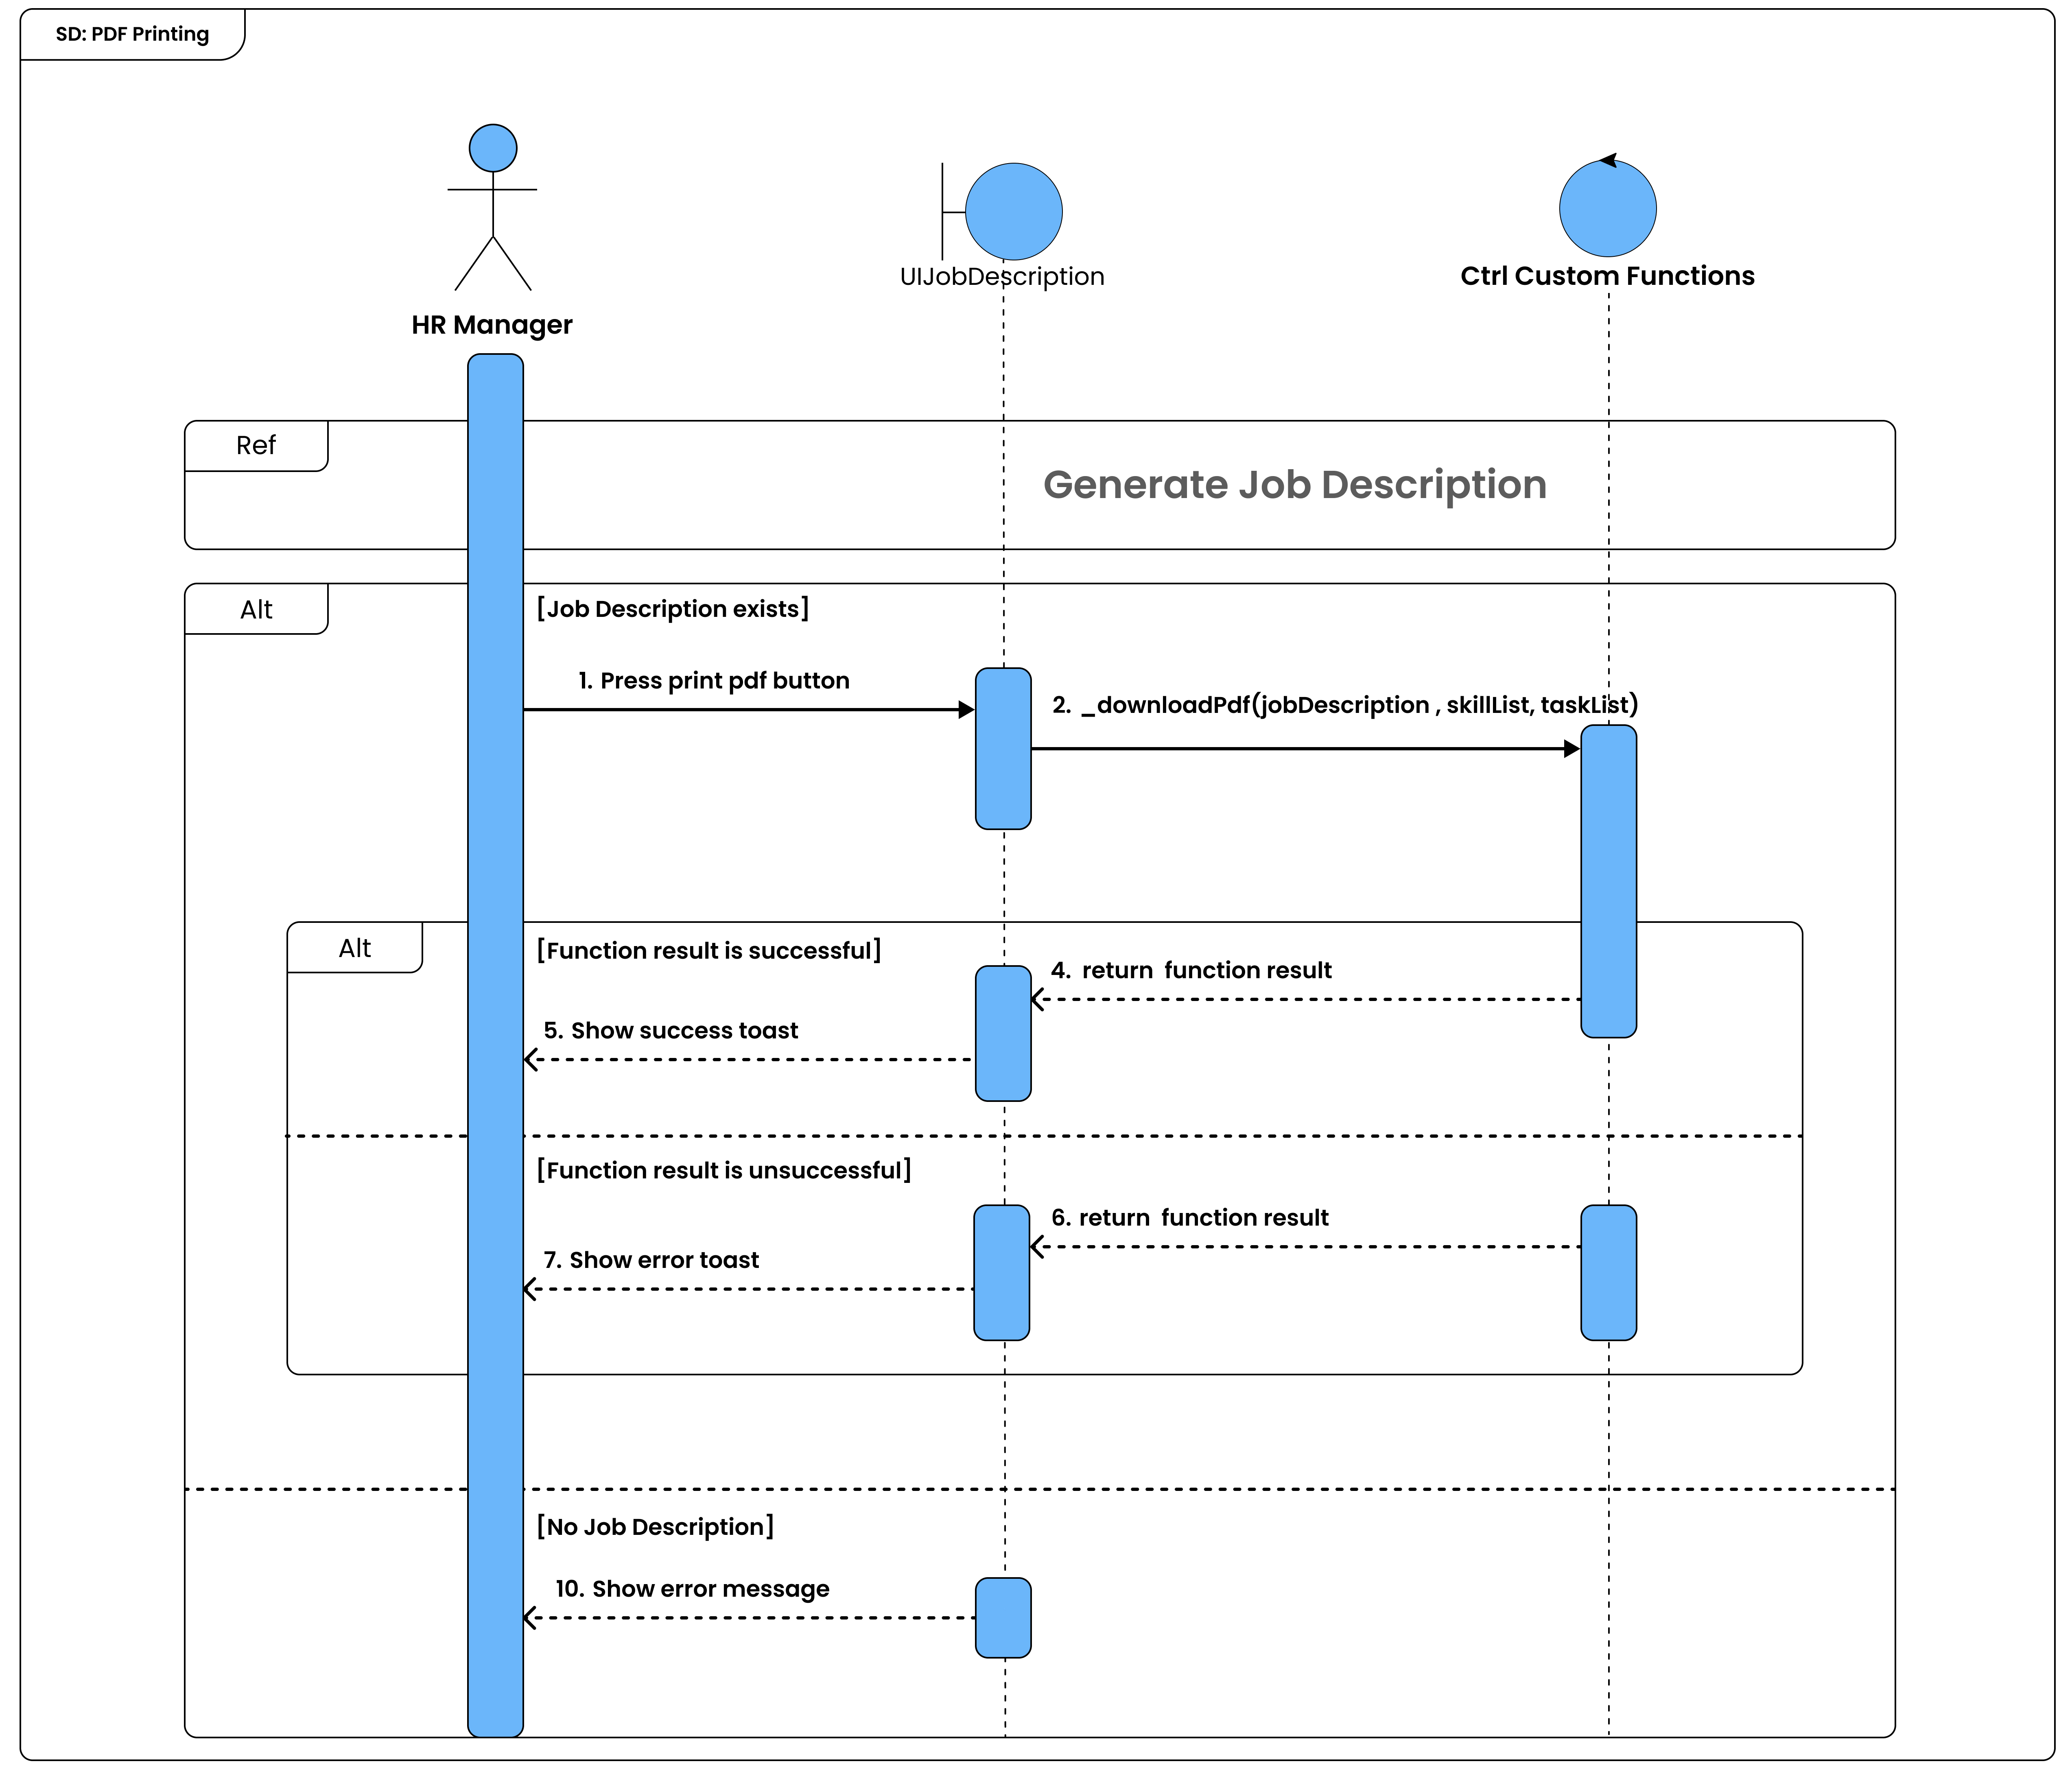
\includegraphics[width=1.25\linewidth]{src/assets/images/SD-PDF-Print.jpg}}
    \caption{ Sequence Diagram for the Print the Nested Skills and Tasks to a PDF Use-Case }
    \label{fig:UseCase2Sprint3_Sequence_Diagram}
\end{figure}

\subsection*{Description}
The sequence diagram shows how a PDF containing job description, skills, and tasks is created. The HR Manager initiates the process by clicking "Generate PDF" after a job description is formulated. This triggers the "downloadPDF" function in FlutterFlow, which requests the Render service to process the data. Render communicates with Puppeteer, a Node.js API, which generates the PDF. The PDF is then sent back through Render to FlutterFlow, enabling the HR Manager to download it. The process ends with a success message or an error message if issues occur.

\subsubsection{Use Case 3: Interact with a Chatbot for Guidance} 

\begin{figure}[H]
    \centering
    \makebox[\textwidth]{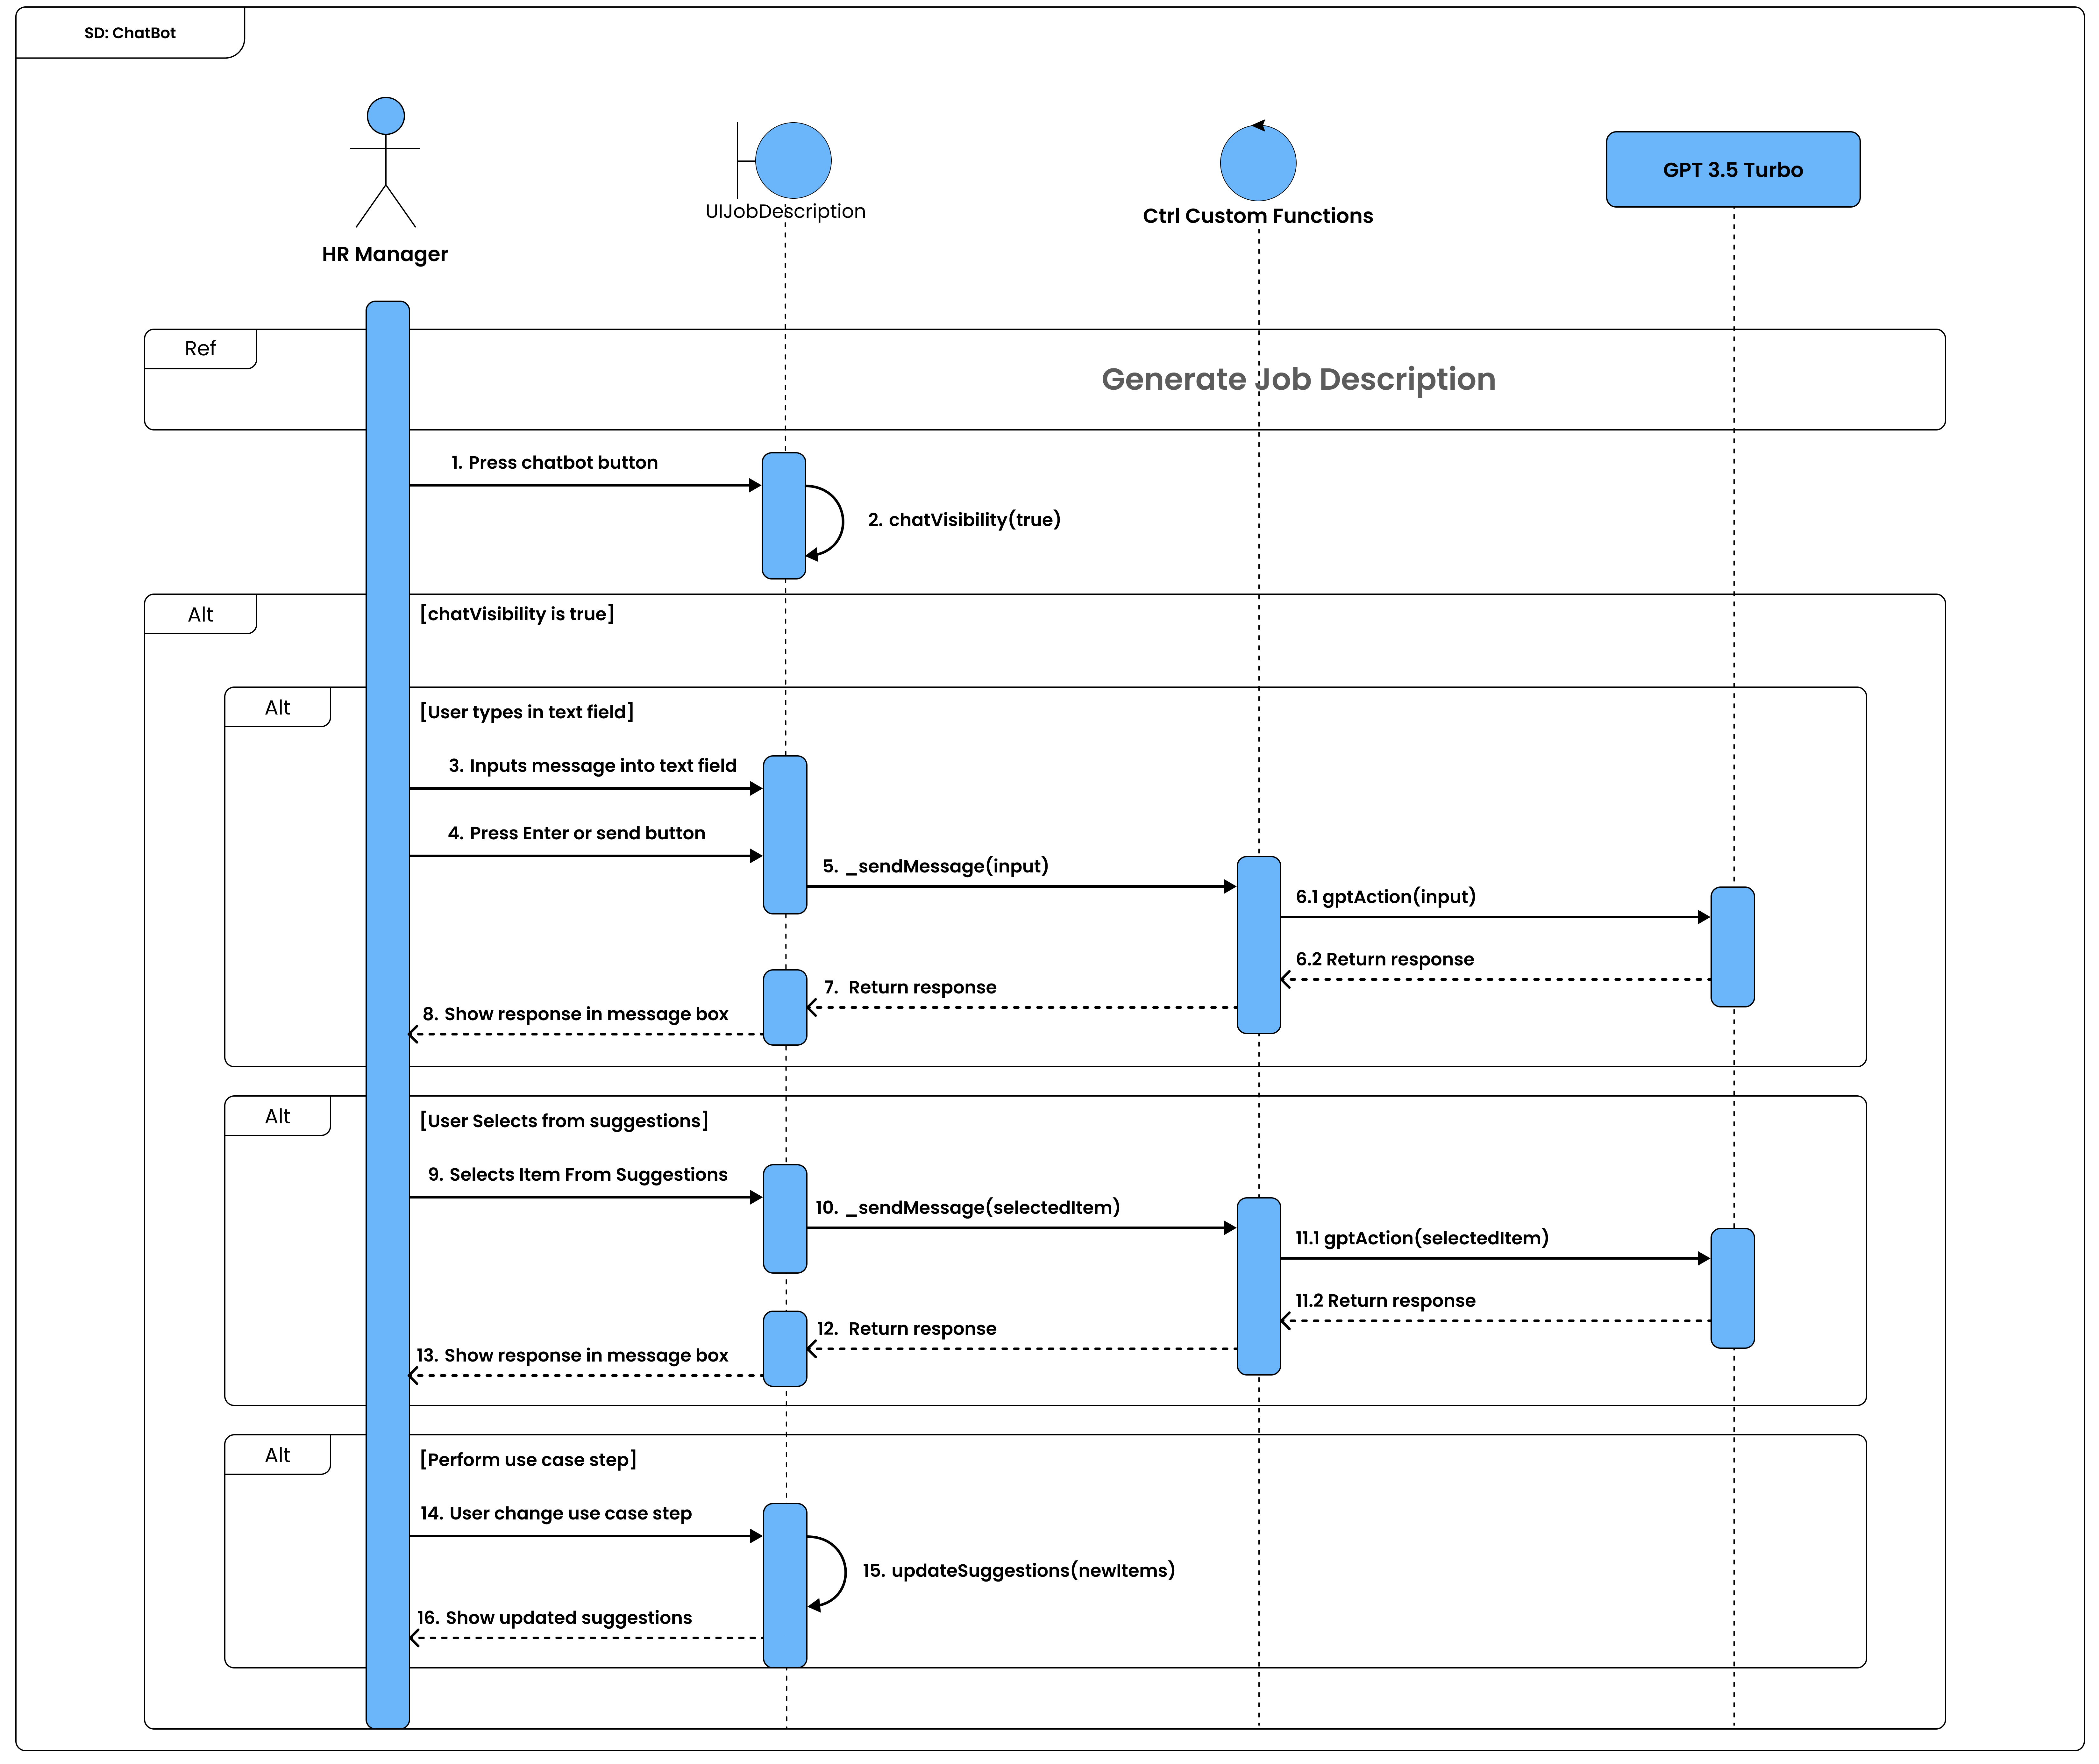
\includegraphics[width=1.2\linewidth]{src/assets/images/SD-Chat-Bot.jpg}}
    \caption{ Sequence Diagram for the Interact with a Chatbot for Guidance Use-Case }
    \label{fig:UseCase3Sprint3_Sequence_Diagram}
\end{figure}

\subsection*{Description}
The sequence diagram delineates the HR Manager's interaction with the chatbot via the GPT-3.5 Turbo model API. It commences with the HR Manager adjusting the chatbot's visibility using the "Chat Visibility" button in the FlutterFlow interface. If the chatbot is enabled, the HR Manager interacts by either typing a message in the TextField and sending it or selecting from the suggestions box. Both these actions prompt the "sendMessage" function which communicates with the GPT-3.5 Turbo model API. The model processes the input and generates a response, displayed in the message box. As actions are performed, the suggestions update to offer relevant prompts. The chatbot is hidden once the "Chat Visibility" button is toggled off.

\section{Implementation}
In this sprint, the main goal was to enhance the job description definition feature and facilitate better communication of the defined job descriptions. This involved creating functionalities for users to email job descriptions, print to PDF, and interact with a chatbot.

\subsection{Email Job Descriptions} 
The first step was to develop a process to email job descriptions. This involved creating a feature that allows HR Managers to input candidate email addresses and send the generated job descriptions directly from the system.

The backend functionality was then developed to handle the email sending process. This involved setting up an email server and writing the necessary server-side code to handle the email sending process.


\begin{figure}[H]
    \centering
    \makebox[\textwidth]{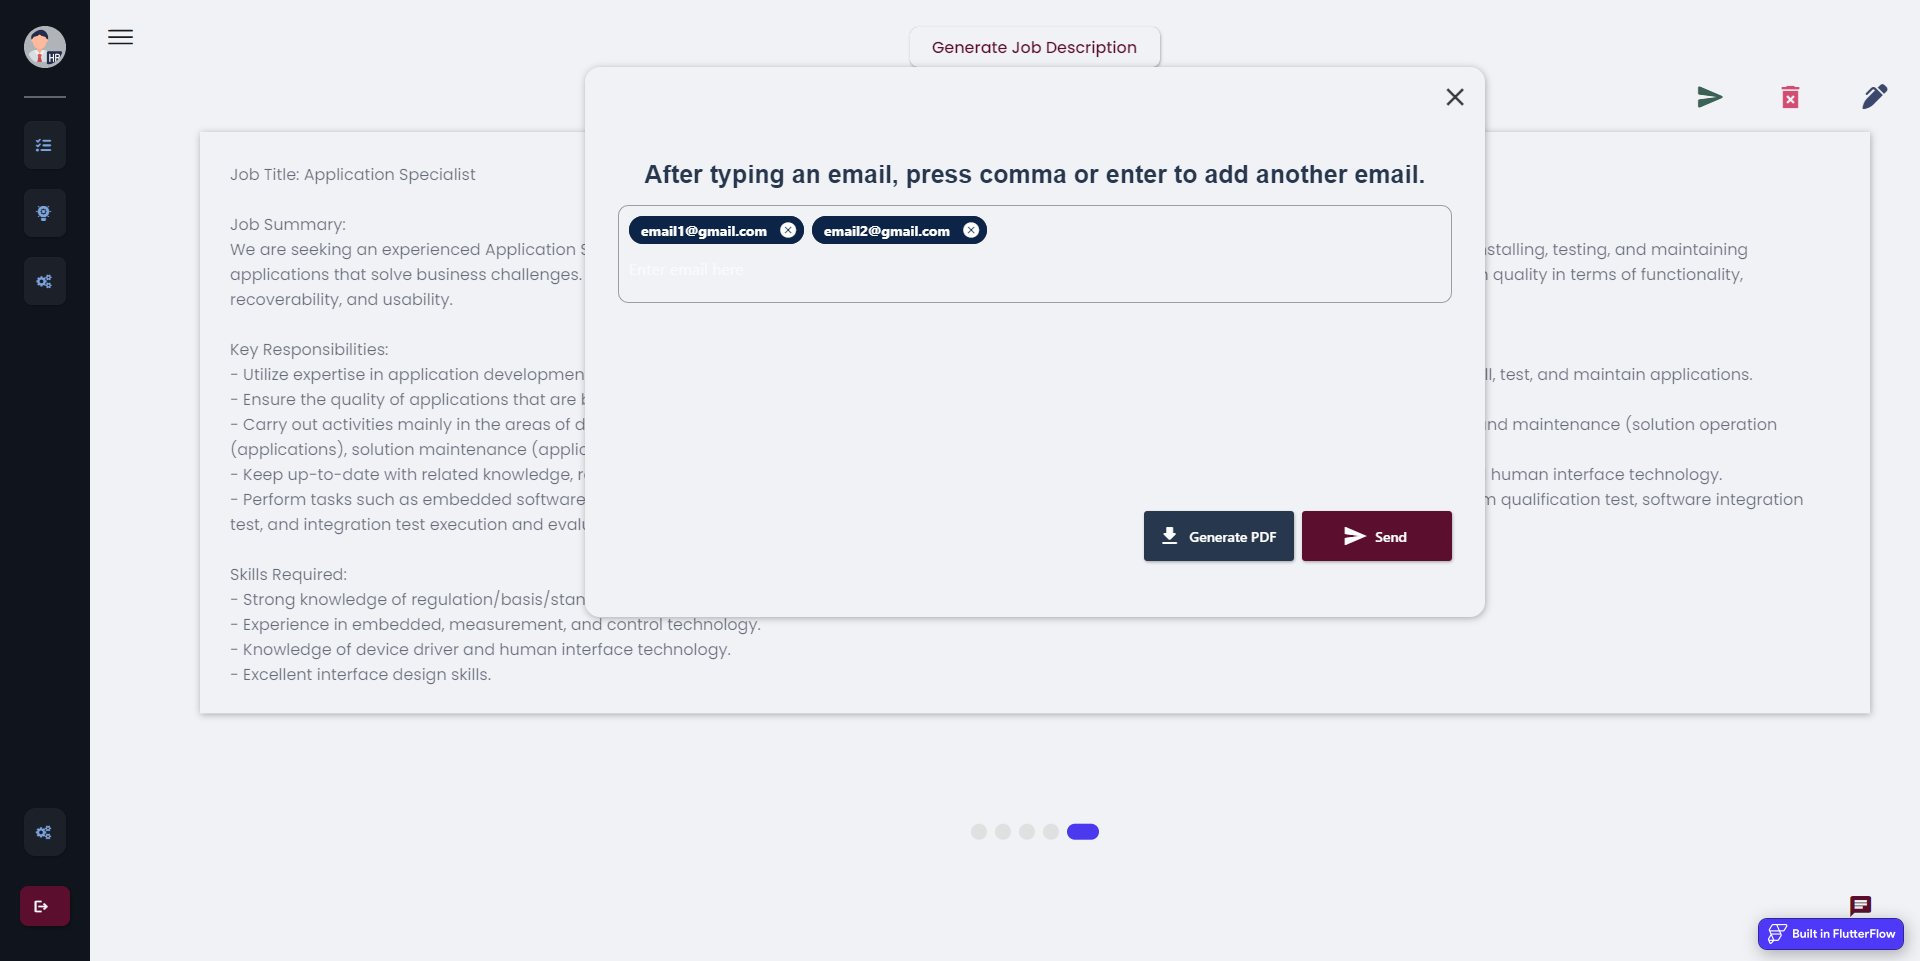
\includegraphics[width=1.2\linewidth]{src/assets/images/sprint3_EmailModal.PNG}}
    \caption{ Email Job Descriptions overview page}
    \label{fig:Email-Job-Descriptions-overview-page}
\end{figure}


\subsection{Print to PDF} 
The next step was to develop a process to convert selected skills and tasks to a PDF. This involved creating a feature that allows HR Managers to generate a PDF of the job description, including the nested skills and tasks, for documentation or offline use.

The backend functionality was then developed to handle the PDF generation process. This involved writing server-side code to convert the job description data into a PDF format.

\begin{figure}[H]
    \centering
    \makebox[\textwidth]{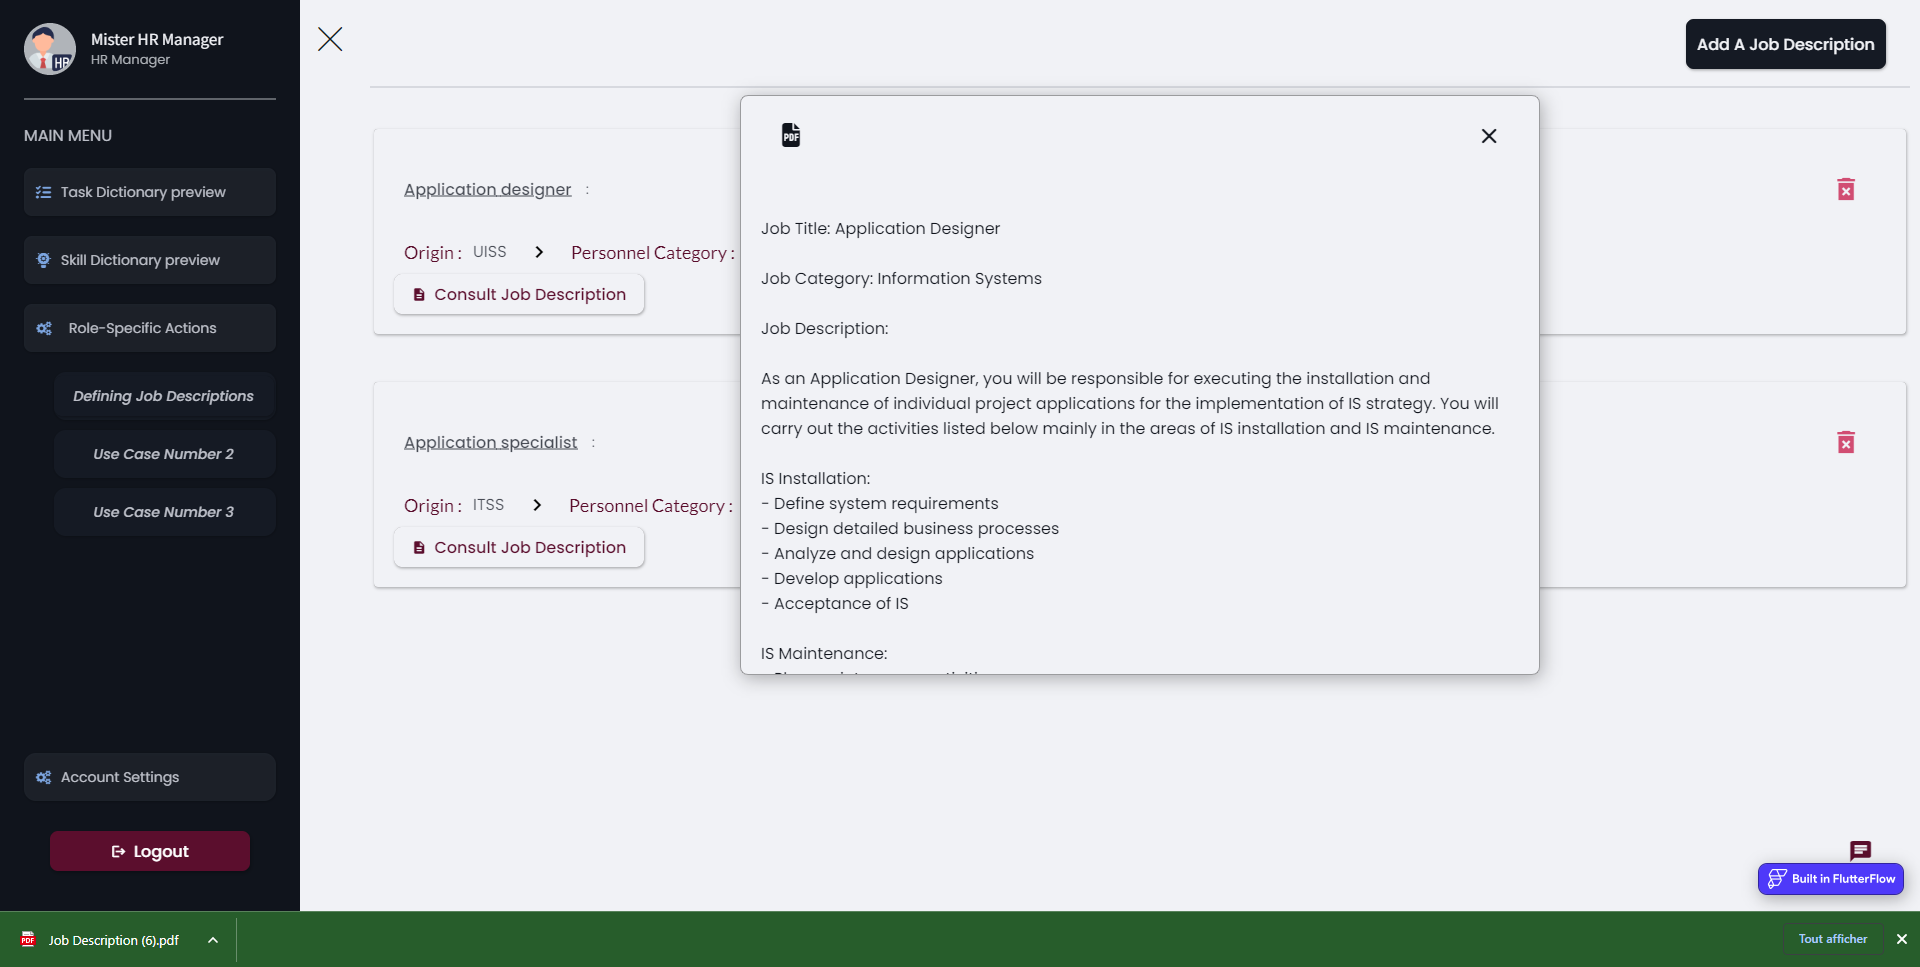
\includegraphics[width=1.2\linewidth]{src/assets/images/sprint3_PDFFeature.PNG}}
    \caption{ Print to PDF overview page }
    \label{fig:Print-to-PDF-overview-page}
\end{figure}


\subsection{Chatbot Integration} 
The final step was to develop a chatbot using GPT-3. This involved creating a chatbot that can understand user queries and provide guidance on the job description creation process.

The chatbot was then integrated into the system. This involved writing server-side code to handle the interaction between the chatbot and the user, and ensuring that the chatbot can access the necessary data to provide accurate responses.




\begin{figure}[H]
    \centering
    \makebox[\textwidth]{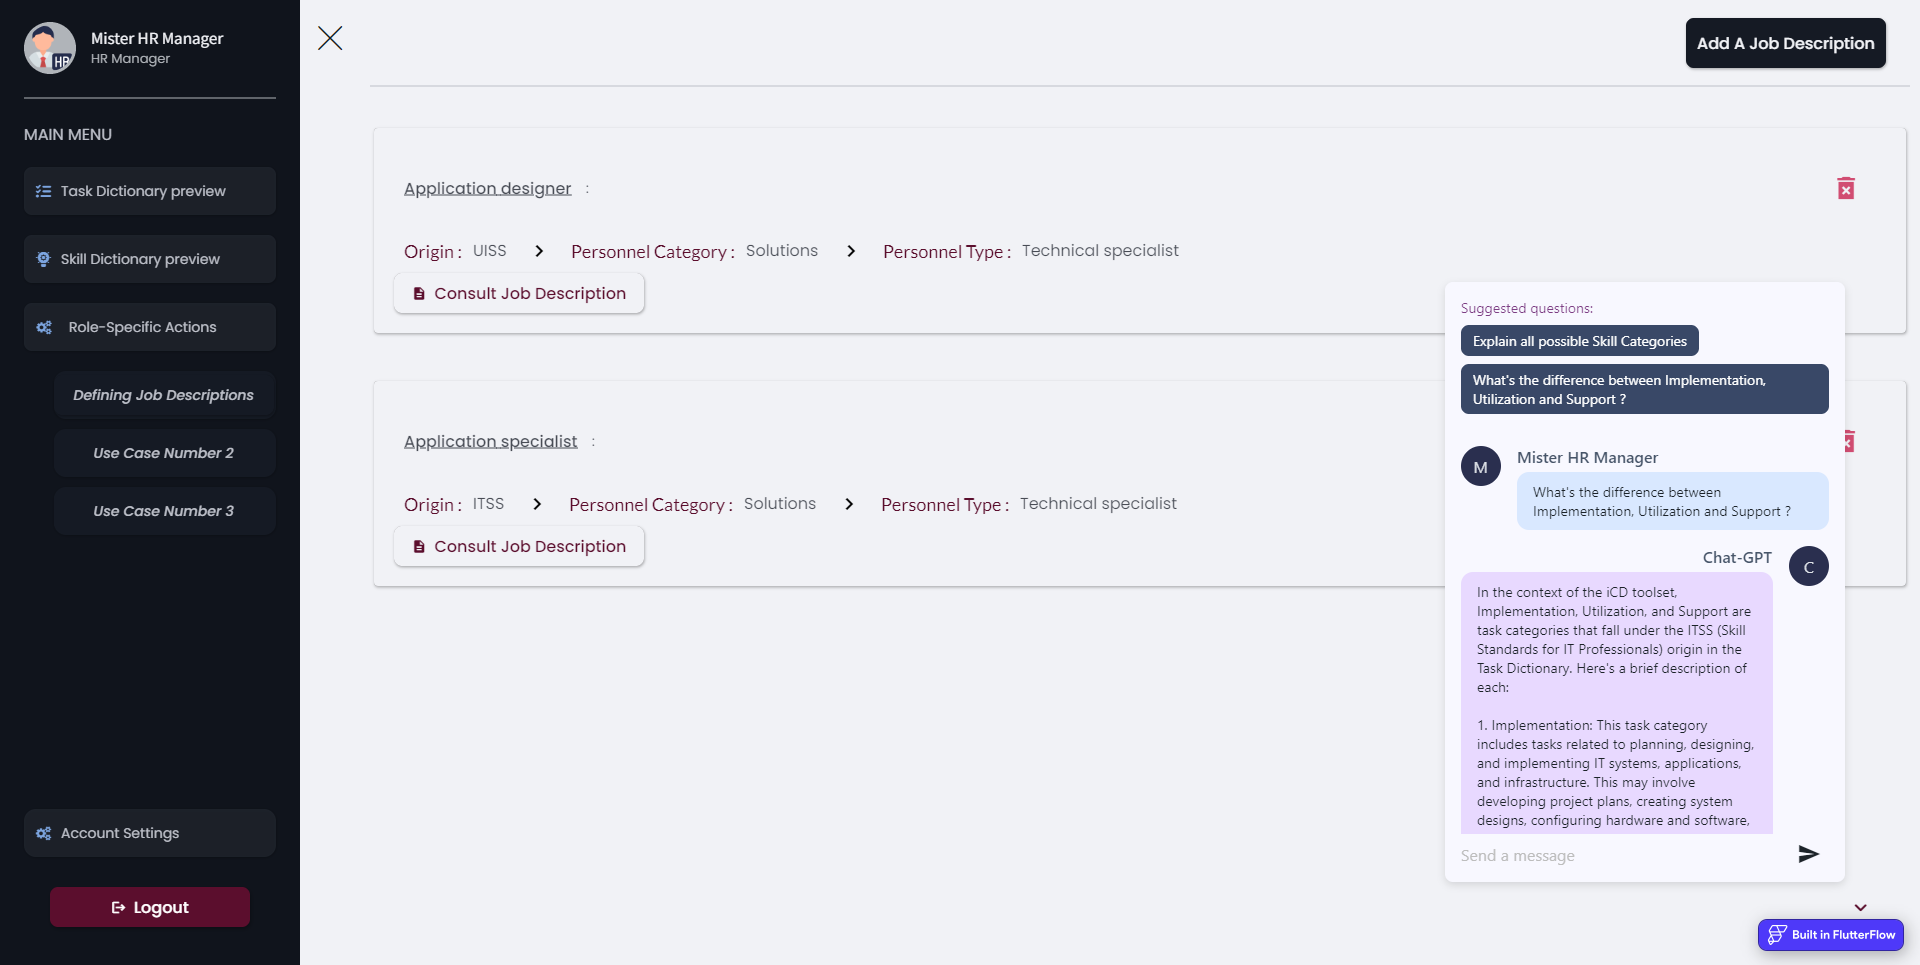
\includegraphics[width=1.2\linewidth]{src/assets/images/sprint3_ChatBotPart2.PNG}}
    \caption{ Chatbot Integration overview page}
    \label{fig:Chatbot-Integration-Vue2-overview-page}
\end{figure}


\subsection{Integration and Testing} 
Once all these features were developed, they were integrated into the overall system. This involved ensuring that they interacted correctly with other system features and data, and that they provided a smooth and intuitive user experience.
Finally, thorough testing was conducted to ensure that all the features worked as expected. This involved testing each feature individually and as part of the overall system, and fixing any bugs or issues that were identified.
$ \rightarrow $ This concludes the implementation of the third sprint. The successful completion of this sprint enhanced the utility of the job description definition feature and made it more convenient for HR Managers to communicate the defined job descriptions.